% An open browser simulator of a gated weir and its river basin: Bendung Perjaya on the Komering River, Sumatra
% Build: make   (runs the engines, writes numbers.tex, tab_*.tex and figures/, then pdflatex + bibtex)
% Every number in the text is a macro from numbers.tex, generated by scripts/build.py. Do not type numbers here.
\documentclass[10pt,a4paper,twocolumn]{extarticle}
\usepackage[T1]{fontenc}
\usepackage[utf8]{inputenc}
\usepackage{mathptmx}
\usepackage[scaled=0.9]{helvet}
\usepackage{courier}
\usepackage[a4paper,left=16mm,right=16mm,top=17mm,bottom=19mm,columnsep=6mm]{geometry}
\usepackage{amsmath}
\usepackage{graphicx}
\usepackage{booktabs}
\usepackage{array}
\usepackage{tabularx}
\usepackage[font=small,labelfont=bf,skip=4pt]{caption}
\usepackage{xcolor}
\usepackage{microtype}
\usepackage{enumitem}
\usepackage{titlesec}
\usepackage[numbers,sort&compress]{natbib}
\usepackage{tikz}
\usetikzlibrary{arrows.meta,positioning}
\usepackage[hidelinks]{hyperref}
\usepackage{url}
\urlstyle{same}

% GENERATED by paper/scripts/build.py from paper/results/results.json. Do not edit.
\newcommand{\CatchArea}{4,305}
\newcommand{\CatchGrid}{4,318}
\newcommand{\CatchGridErrPct}{$+$0.3}
\newcommand{\RainAnnual}{2,815}
\newcommand{\RunoffShare}{0.51}
\newcommand{\RepYearFirst}{1991}
\newcommand{\RepYearLast}{2025}
\newcommand{\RepNYears}{35}
\newcommand{\QmeanPub}{203.1}
\newcommand{\QmeanRep}{195.6}
\newcommand{\QmeanErrPct}{$-$3.7}
\newcommand{\QmeanAbsErrPct}{4}
\newcommand{\RmsMeanPct}{15}
\newcommand{\MaxMeanErrPct}{$-$29}
\newcommand{\MaxMeanErrMonth}{Sep}
\newcommand{\RmsQeightyPct}{19}
\newcommand{\DryQeightyLoPct}{0}
\newcommand{\DryQeightyHiPct}{$+$18}
\newcommand{\DryQeightyAbsPct}{18}
\newcommand{\MaxQeightyErrPct}{$+$33}
\newcommand{\MaxQeightyErrMonth}{Feb}
\newcommand{\AnnMaxLo}{283}
\newcommand{\AnnMaxHi}{612}
\newcommand{\PubQtwo}{917}
\newcommand{\PubQhundred}{1,939}
\newcommand{\PubLargest}{1,438}
\newcommand{\GlofasCorr}{0.94}
\newcommand{\GlofasMean}{217}
\newcommand{\GlofasYearFirst}{1997}
\newcommand{\ClimQmean}{188}
\newcommand{\BucketSmax}{117}
\newcommand{\BucketKfast}{11.6}
\newcommand{\BucketKslow}{152}
\newcommand{\BucketGwShare}{0.69}
\newcommand{\BucketEtFactor}{1.21}
\newcommand{\BucketFc}{0.92}
\newcommand{\BucketSlowExp}{1.06}
\newcommand{\DesignTp}{3}
\newcommand{\DesignShape}{4}
\newcommand{\DriestYear}{1997}
\newcommand{\DriestRain}{1,608}
\newcommand{\PondNormal}{79.70}
\newcommand{\DHW}{81.00}
\newcommand{\DesignQ}{2,200}
\newcommand{\BalanceErr}{$8\times10^{-6}$}
\newcommand{\PondHeldTo}{1,660}
\newcommand{\PondOverFrom}{2,370}
\newcommand{\DesignPondAuto}{80.71}
\newcommand{\DesignTailAuto}{79.87}
\newcommand{\DesignFreeboard}{0.29}
\newcommand{\QhundredPondAuto}{80.23}
\newcommand{\DesignPondOpen}{80.85}
\newcommand{\DesignTailOpen}{80.00}
\newcommand{\WavePondPeak}{80.75}
\newcommand{\WaveVolume}{645}
\newcommand{\WaveDepth}{150}
\newcommand{\MaxPondJump}{0.01}
\newcommand{\SolveMs}{1.2}
\newcommand{\IntakeTarget}{81}
\newcommand{\IntakeDesign}{91.68}
\newcommand{\IntakeMax}{101}
\newcommand{\EnvFlow}{35}
\newcommand{\TailBed}{74.23}
\newcommand{\TailWidth}{200}
\newcommand{\TailN}{0.035}
\newcommand{\TailSlope}{0.00042}
\newcommand{\FirstOpening}{0.30}
\newcommand{\RefTail}{78.2}
\newcommand{\RefFlow}{1,175}
\newcommand{\FirstWetQ}{1,410}
\newcommand{\MinDepth}{0.3}
\newcommand{\FloodAreaDesign}{5.5}
\newcommand{\FloodAreaUpDesign}{3.6}
\newcommand{\FloodAreaDownDesign}{1.9}
\newcommand{\FloodBldDesign}{86}
\newcommand{\FloodRoadDesign}{1.1}
\newcommand{\FloodCropDesign}{265}
\newcommand{\FloodRiseBelowDesign}{1.67}
\newcommand{\FloodRiseAboveDesign}{1.01}
\newcommand{\FloodAreaQhundred}{3.3}
\newcommand{\FloodBldQhundred}{56}
\newcommand{\SensAreaLo}{4.3}
\newcommand{\SensAreaHi}{8.6}
\newcommand{\SensBldLo}{78}
\newcommand{\SensBldHi}{106}
\newcommand{\ExtentMs}{24}
\newcommand{\WideCols}{2,040}
\newcommand{\WideCellM}{93}
\newcommand{\FineCols}{1,260}
\newcommand{\FineRows}{1,440}
\newcommand{\FineCellM}{31}
\newcommand{\IrrArea}{62,536}
\newcommand{\IrrEff}{0.65}
\newcommand{\PeakDR}{1.11}
\newcommand{\PeakHM}{May II}
\newcommand{\PeakDemand}{69.7}
\newcommand{\PeakDRPub}{1.1}
\newcommand{\PeakDemandPub}{68.8}
\newcommand{\PeakDRErrPct}{1}
\newcommand{\WorstYear}{1997}
\newcommand{\LeastDryShortDays}{24}
\newcommand{\NDryYears}{4}
\newcommand{\WorstShortDays}{88}
\newcommand{\WorstShortVol}{121}
\newcommand{\WorstShortPct}{13}
\newcommand{\MeanYearShortDays}{0}
\newcommand{\YearDemandVol}{942}
\newcommand{\EnvBreachDays}{0}
\newcommand{\SedYieldMt}{5.02}
\newcommand{\SedUnscaledMt}{14.2}
\newcommand{\SedScale}{0.35}
\newcommand{\SedRatingA}{0.053}
\newcommand{\SedRatingB}{2.52}
\newcommand{\SedIntakeKt}{272}
\newcommand{\SedTrapKt}{88}
\newcommand{\SedTrapPct}{32}
\newcommand{\SedIntakePct}{5.4}
\newcommand{\SedFlushes}{14}
\newcommand{\SedInterval}{130}
\newcommand{\SedStorage}{6,300}
\newcommand{\SedCmean}{697}
\newcommand{\SedBasins}{5}
\newcommand{\SedFlushHours}{4}
\newcommand{\SedFlushAtPct}{80}
\newcommand{\TDCatch}{1,158}
\newcommand{\TDCatchPub}{1,158}
\newcommand{\TDCatchErrPct}{$-$0.03}
\newcommand{\TDCrest}{326}
\newcommand{\TDHeight}{89}
\newcommand{\TDHeightPub}{122}
\newcommand{\TDLen}{1,104}
\newcommand{\TDLenPub}{950}
\newcommand{\TDVol}{81}
\newcommand{\TDVolPub}{129}
\newcommand{\TDVolPct}{62}
\newcommand{\TDArea}{2.8}
\newcommand{\TDFillDays}{17}
\newcommand{\TDInflow}{50}
\newcommand{\SelVol}{170}
\newcommand{\SelArea}{8.2}
\newcommand{\SelLen}{1,254}
\newcommand{\SelCatch}{1,219}
\newcommand{\SelHeight}{40}
\newcommand{\SelFillDays}{31}
\newcommand{\CatchMs}{10}
\newcommand{\CurveMs}{3}
\newcommand{\NParams}{158}
\newcommand{\NParamsS}{67}
\newcommand{\NParamsC}{32}
\newcommand{\NParamsR}{3}
\newcommand{\NParamsA}{56}
\newcommand{\NParamsAPct}{35}
\newcommand{\NFacts}{119}
\newcommand{\NFactsS}{88}
\newcommand{\NSources}{49}
\newcommand{\DatumOffset}{3.2}
\newcommand{\ResultsDate}{2026-11-27}
\newcommand{\NBuildings}{719,156}
\newcommand{\NRainPoints}{12}
\newcommand{\GlofasYearLast}{2025}
\newcommand{\LocCode}{23,049}
\newcommand{\LocEngine}{3,698}
\newcommand{\NModules}{90}
\newcommand{\NTestFiles}{20}
\newcommand{\NTargets}{40}
\newcommand{\NTests}{215}
\newcommand{\NPass}{212}
\newcommand{\NFail}{0}
\newcommand{\NSkip}{3}
\newcommand{\NParamsShown}{53}

\makeatletter\newcommand{\rows}[1]{\@@input #1.tex }\makeatother % table rows made by scripts/build.py
\newcommand{\cms}{m$^3$/s}
\newcommand{\kmsq}{km$^2$}
\newcommand{\Mm}{million~m$^3$}
\newcommand{\RepoURL}{https://github.com/lucacadalora/perjaya-weir-simulator}
\newcommand{\DemoURL}{https://perjaya.vantis.sh}

\titleformat{\section}{\normalfont\large\bfseries}{\thesection}{0.6em}{}
\titleformat{\subsection}{\normalfont\normalsize\bfseries}{\thesubsection}{0.6em}{}
\titlespacing*{\section}{0pt}{9pt plus 2pt minus 2pt}{3pt}
\titlespacing*{\subsection}{0pt}{6pt plus 2pt minus 1pt}{2pt}
\setlength{\parskip}{0pt}
\setlength{\parindent}{1em}
\setlength{\textfloatsep}{9pt plus 2pt minus 2pt}
\setlength{\dbltextfloatsep}{9pt plus 2pt minus 2pt}
\setlength{\floatsep}{8pt plus 2pt minus 2pt}
\setlength{\abovedisplayskip}{4pt plus 1pt minus 1pt}
\setlength{\belowdisplayskip}{4pt plus 1pt minus 1pt}
\setlist{nosep,leftmargin=1.2em}
\renewcommand{\bibfont}{\footnotesize}
\setlength{\bibsep}{1pt plus 0.5pt}
\hypersetup{pdftitle={An open browser simulator of a gated weir and its river basin: Bendung Perjaya on the Komering River, Sumatra},
  pdfauthor={Luca Cada Lora}, pdfsubject={Open-source hydrological and hydraulic simulation in the browser}}

\title{\vspace{-8mm}\Large\bfseries An open browser simulator of a gated weir and its river basin:\\
Bendung Perjaya on the Komering River, Sumatra}
\author{\normalsize Luca Cada Lora\\[1pt] \small Jatevo Labs Limited}
\date{\small Preprint, 27 November 2026 \quad$\cdot$\quad code and data: \url{\RepoURL}}

\begin{document}
\twocolumn[
\maketitle
\vspace{-6mm}
\begin{center}
\begin{minipage}{0.88\textwidth}
\small
\noindent\textbf{Abstract.}
Barrages that feed large irrigation schemes are run from manuals and consultants' reports that few people outside the
operating office read, and the models that describe them usually need desktop software and a trained user. We present
an open-source simulator that runs entirely in a web browser and reproduces, at indicative accuracy, the working of
Bendung Perjaya, the gated weir that diverts the Komering River in South Sumatra, Indonesia, into a command area of
\IrrArea~ha. A chain of eight small calculation engines turns daily basin rain into river flow; splits that flow
between seven flood gates, three scouring sluices and the canal intake under an automatic or a manual rule; maps the
ground flooded beyond the normal river and counts what the water reaches; balances irrigation demand against supply;
follows sediment through five settling basins; and lets the user place a dam of their own anywhere in the
\CatchArea~\kmsq{} catchment. Every constant sits in one data file with its source and a status letter;
\NParamsA{} of \NParams{} are marked as assumed. Against the published tables it was fitted to, the modelled mean flow is within
\QmeanAbsErrPct~\%, monthly means within \RmsMeanPct~\% (root mean square) and dry-season dependable flows within
\DryQeightyAbsPct~\%; the design flood of \DesignQ~\cms{} passes with the pond \DesignFreeboard~m below design high
water; peak irrigation demand is \PeakDR{} against a published \PeakDRPub~l/s/ha. A 30~m surface model limits the
flood maps and reservoir volumes, and no gauge record was available for calibration: the results are a model, not a
survey or a forecast. Code, data and the scripts that produce every number in this paper are public under the MIT
licence.
\end{minipage}
\end{center}
\vspace{4mm}
]

\section{Introduction}

Indonesia irrigates much of its rice from run-of-river barrages (\emph{bendung gerak}): gated weirs that hold a pond
just high enough to push water into a canal, with no reservoir behind them. How such a structure behaves over a year,
how its gates answer a flood, when the canal runs short and what the river below keeps, is written in operating
manuals and in consultants' reports. The tools that would let someone explore those questions, one-dimensional and
two-dimensional hydraulic models~\citep{brunner2016,bates2000} and catchment models, are desktop programs that need
licensed data, a trained user and hours of set-up. Students, journalists, farmers' groups and local planners
therefore meet the structure only as a photograph and a few headline numbers.

Two lines of earlier work meet here. Flood extent can be mapped quickly from terrain alone by the height above the
nearest drainage~\citep{renno2008,nobre2011}, without solving the flow equations. And water-resources software has
been moving to the web: mostly as server-side models behind a browser front end~\citep{swain2015}, more recently as
libraries that run hydrological analyses in the browser itself~\citep{sit2019,ramirez2022}. Those are general
toolkits. Our aim is narrower and more concrete: one real structure, modelled end to end on the client, with the
provenance of every constant on screen.

The simulator described here is one static web page, no server and no installation,
built on open data only, which puts the real structure at true scale on a three-dimensional map and lets anyone run
it (Fig.~\ref{fig:shots}). The subject is Bendung Perjaya on the Komering River, the headworks of the Komering
irrigation system in South Sumatra. The aim is not to replace an engineering model. It is to make the chain from rain
to gate to field visible and checkable, with each number traceable to a source and each limit stated.

The contributions are: (i)~eight calculation engines, written as pure functions, that cover rain to flow, gate
hydraulics and operation, flood extent, impact, irrigation, sediment and reservoir filling, light enough to run at
interactive speed in a browser; (ii)~a single data file in which every constant carries its source and one of four
status letters, so a reader can see which parts of the answer rest on documents and which on assumption;
(iii)~an evaluation of each engine against published tables, with the errors reported as they are; and (iv)~an open
repository in which a script regenerates every number, table and plot of this paper from the same code the page runs.

\begin{figure*}[t]
\centering
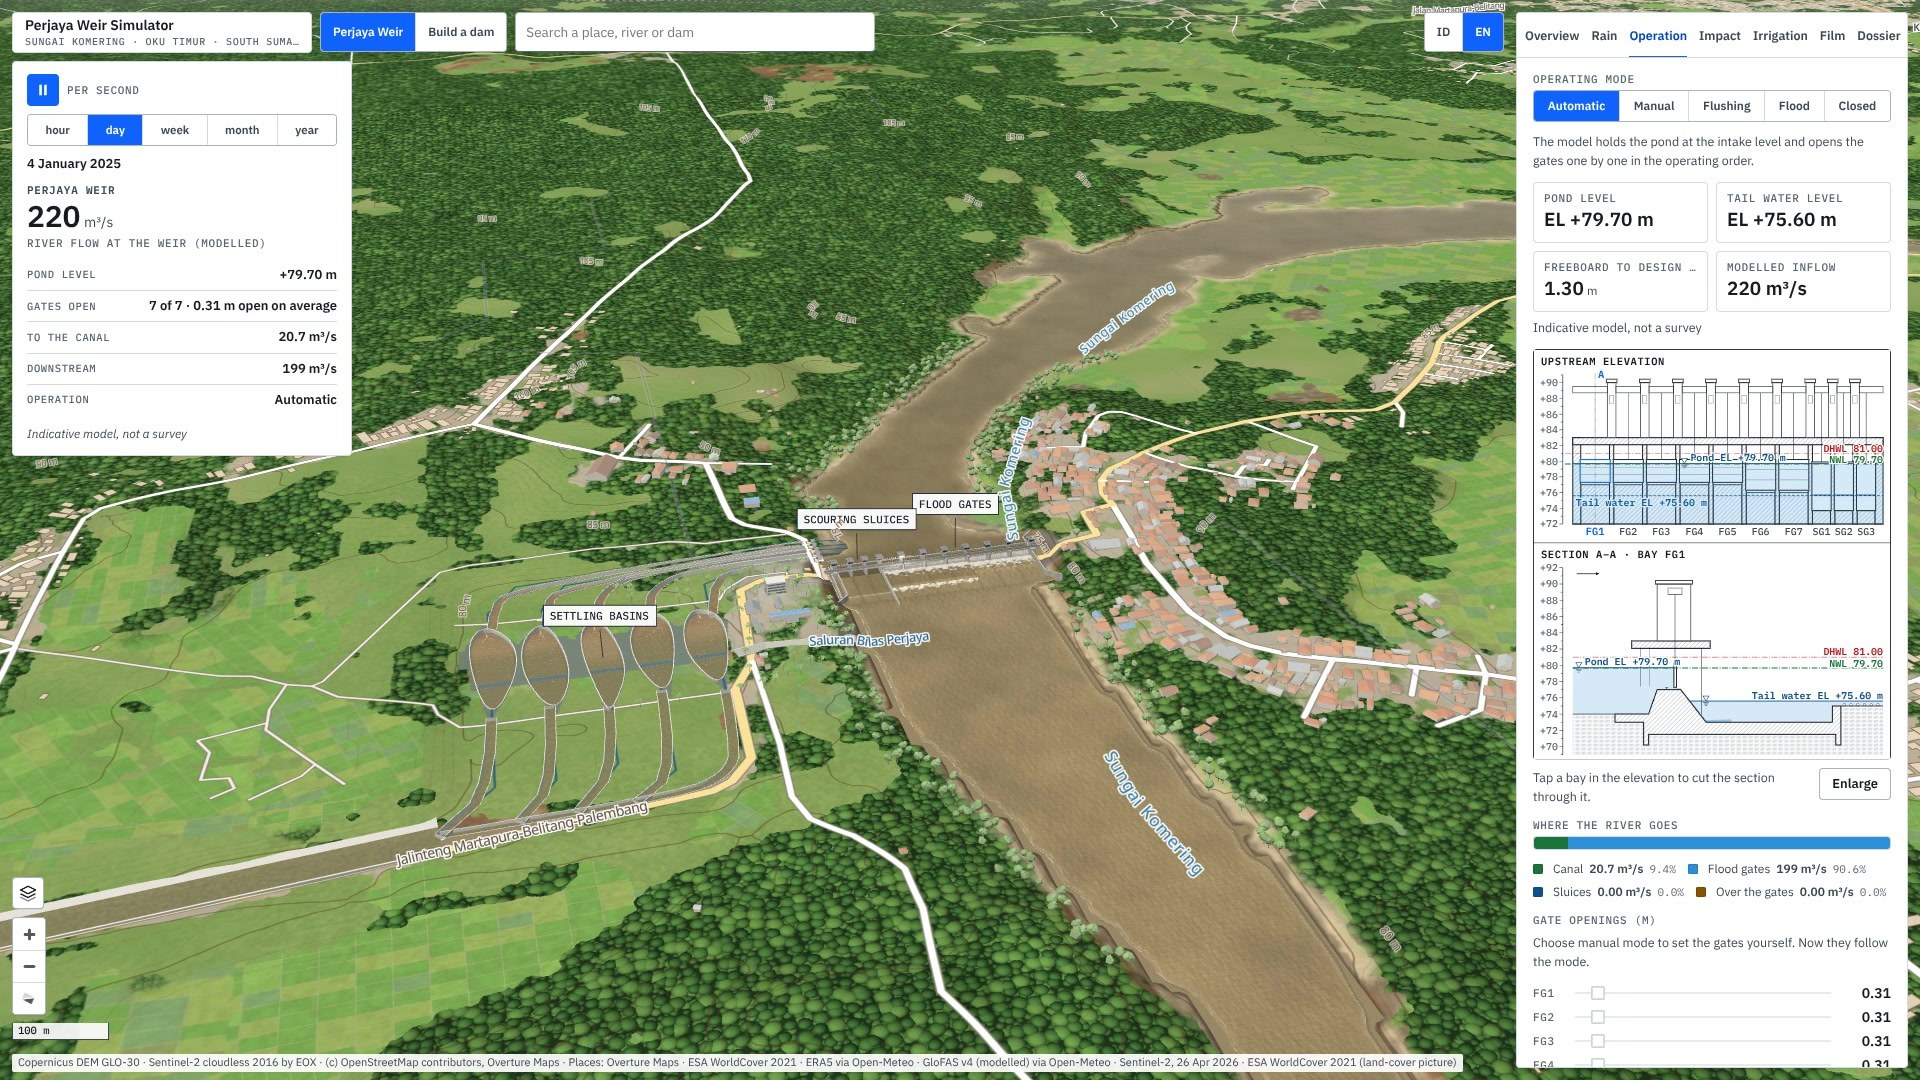
\includegraphics[width=0.495\textwidth]{figures/shot_operation.jpg}\hfill
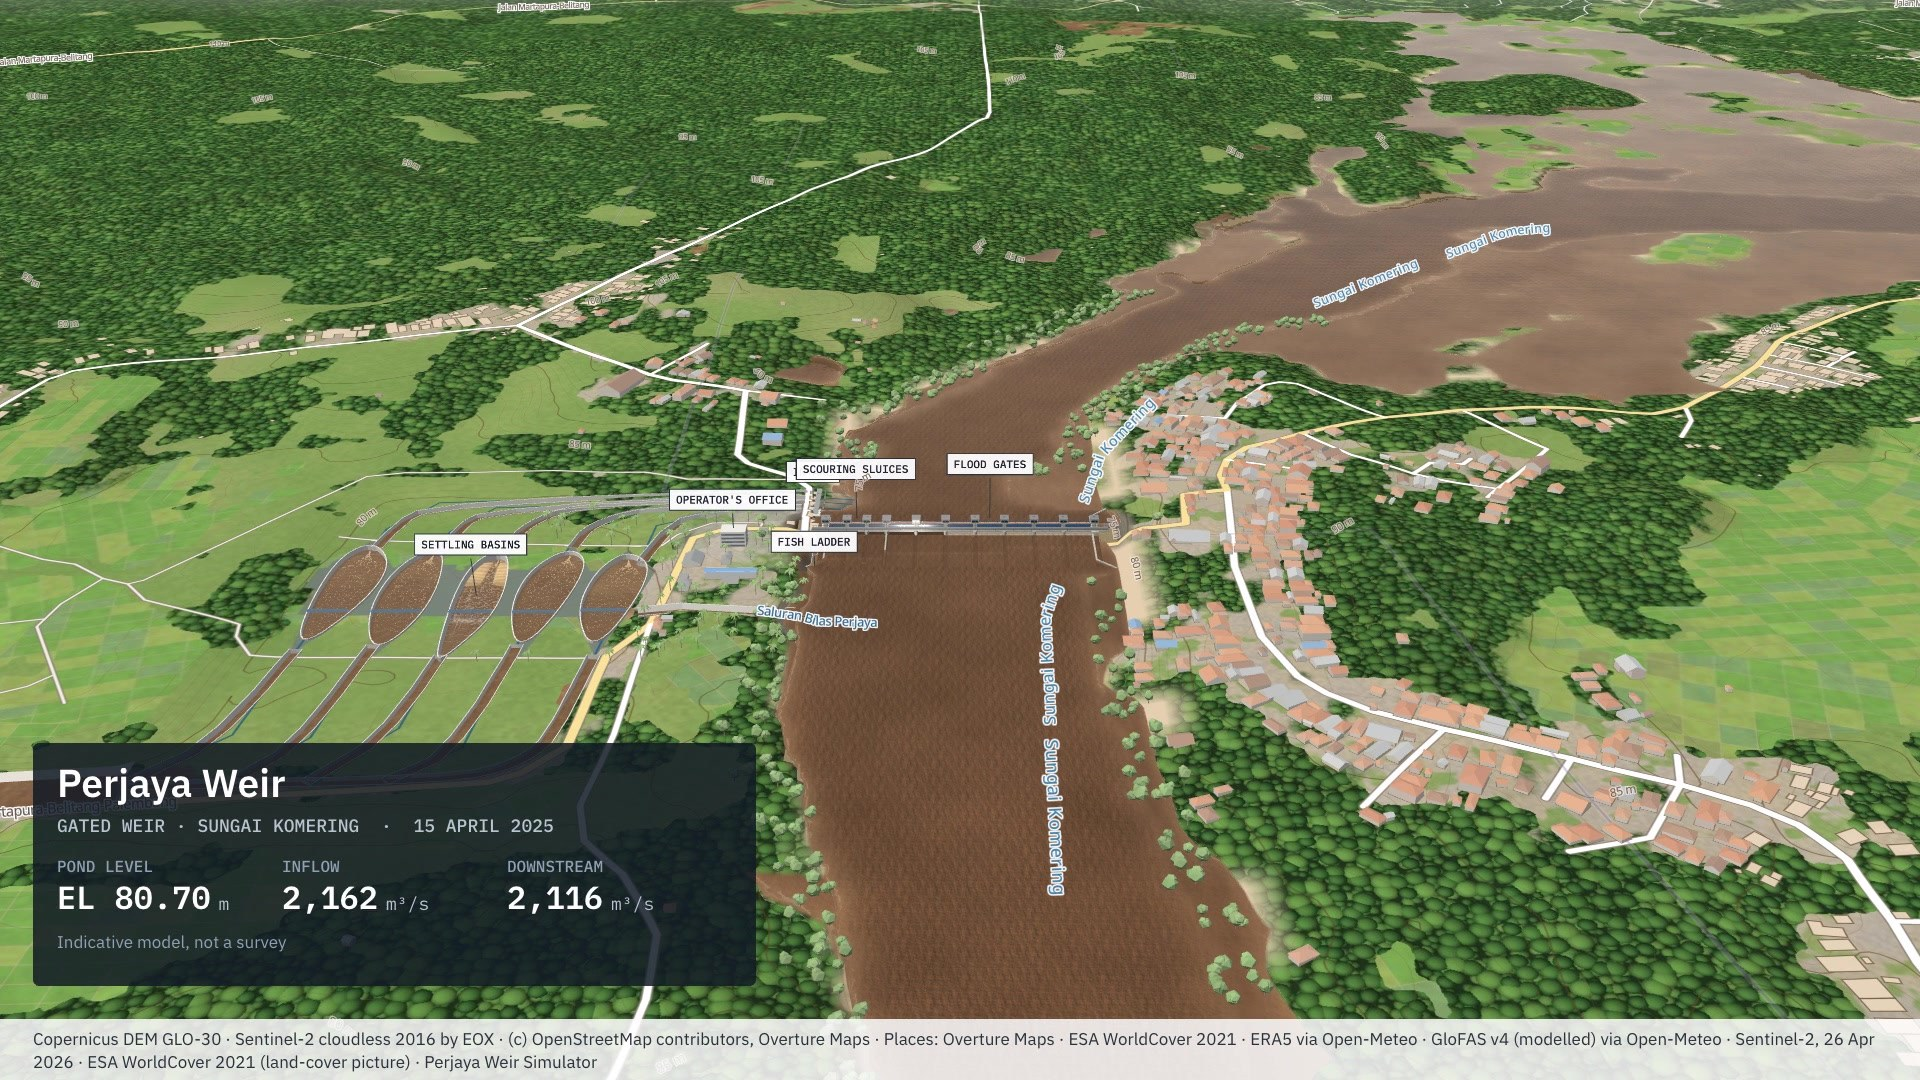
\includegraphics[width=0.495\textwidth]{figures/shot_design_flood.jpg}\\[2pt]
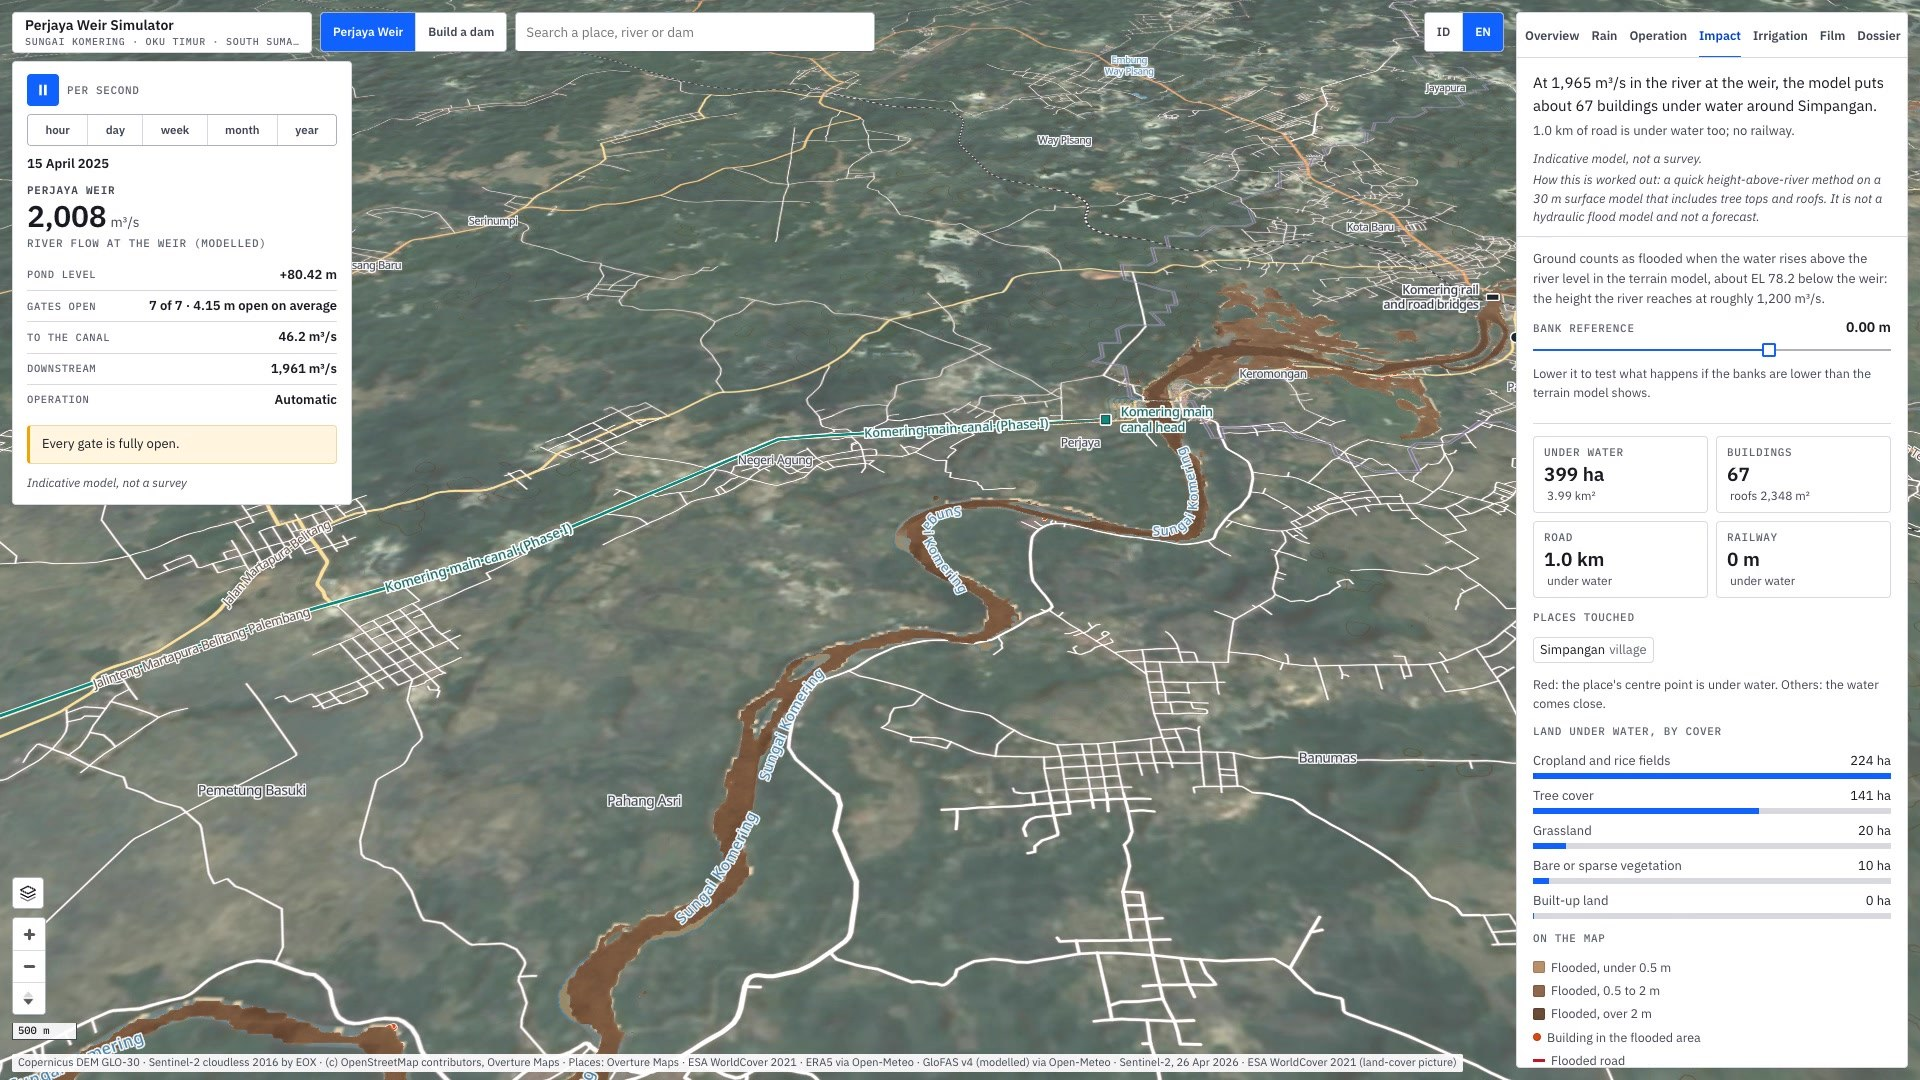
\includegraphics[width=0.495\textwidth]{figures/shot_impact.jpg}\hfill
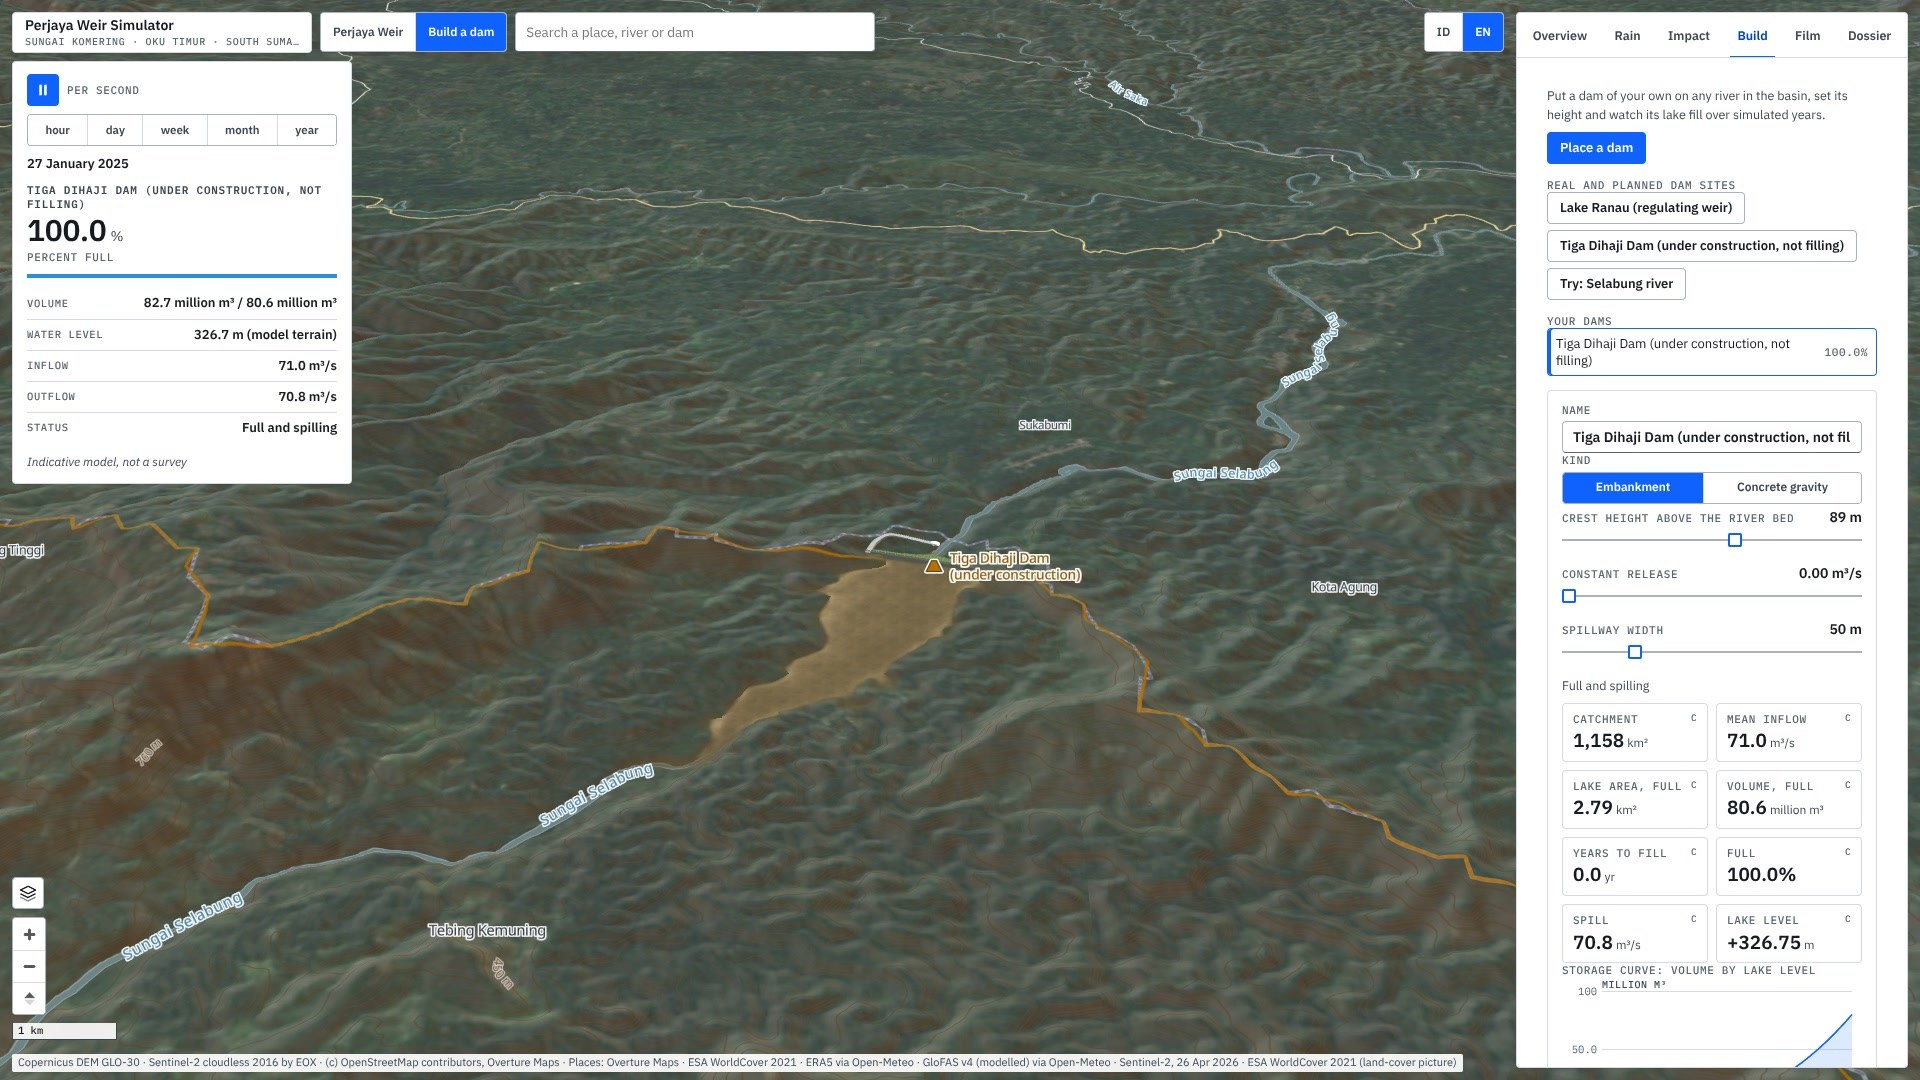
\includegraphics[width=0.495\textwidth]{figures/shot_maker.jpg}
\caption{The simulator in a browser. Top left: the weir at true scale in a mean year, with the operation tab and its
live elevation and section drawing. Top right: the design flood near its peak (film frame without the panels).
Bottom left: the impact tab during that flood, with the flooded ground tinted and counted. Bottom right:
``maker'' mode, a dam placed at the Tiga Dihaji site with its lake, catchment outline and storage curve. Map data
credits are printed in each frame.}
\label{fig:shots}
\end{figure*}

\section{Site and data}

\textbf{The structure.} Bendung Perjaya stands on the Komering near Martapura, about 4~km below the town. Civil works
ran from 1991 to 1996~\citep{jbic2002}. The weir is 215.5~m long with seven flood gates 20~m wide, three scouring
sluices 12.5~m wide on the right bank, a 49.5~m intake with a design capacity of \IntakeDesign~\cms, five settling
basins and a fish ladder~\citep{jica2019}. It holds a normal pond at EL~\PondNormal~m; the design high water is
EL~\DHW~m for a design flood of \DesignQ~\cms, whose return period the documents do not state. The catchment is
\CatchArea~\kmsq{} and the mean flow \QmeanPub~\cms~\citep{jica1982,jica2022}; the legal command area is
\IrrArea~ha~\citep{permen14}. The gate operating order comes from a published evaluation of the gate
operation~\citep{ayun2022}. The operating manual, as-built drawings and gate logs were not available to us, so all
sill, bed and deck levels are assumptions derived from the sourced levels and gate sizes.

\textbf{Open data.} Table~\ref{tab:data} lists the datasets and Fig.~\ref{fig:pipeline} (bands 1 to 3) shows how each
becomes a file the page reads. Terrain comes from the Copernicus GLO-30 surface
model~\citep{copdem}, prepared once into two grids: a ``wide'' grid of \WideCols$\times$\WideCols{} cells of about
\WideCellM~m covering the whole basin, and a ``fine'' grid of \FineCols$\times$\FineRows{} cells of about
\FineCellM~m around the weir. Each grid stores elevation, D8 flow direction~\citep{ocallaghan1984}, upstream area and
height above the nearest drainage~\citep{renno2008,nobre2011}, computed after pit filling and river burning with
pysheds~\citep{bartos2020}. Daily rain and reference evapotranspiration for \RepYearFirst--\RepYearLast{} are ERA5
values~\citep{hersbach2020}, the mean of the cells returned for \NRainPoints{} points across the
basin~\citep{zippenfenig2023}. A second,
independent flow series from the global model GloFAS~\citep{harrigan2020} is kept only for comparison. Land
cover~\citep{zanaga2022}, \NBuildings{} building footprints, roads, rail and place names~\citep{overture2026}
complete the set. Nothing is fetched at run time: all data are static files beside the page.

\begin{table}[t]
\caption{Open datasets behind the simulator. All are redistributed in the repository under their own licences.}
\label{tab:data}
\footnotesize
\begin{tabularx}{\columnwidth}{@{}l>{\raggedright\arraybackslash}X@{}}
\toprule
Dataset & Use in the simulator \\
\midrule
Copernicus DEM GLO-30 & terrain, flow direction, upstream area, height above drainage; map relief \\
ERA5 via Open-Meteo & daily basin rain and reference evapotranspiration, \RepYearFirst--\RepYearLast \\
GloFAS v4 via Open-Meteo & modelled river flow at the weir cell, \GlofasYearFirst--\GlofasYearLast, comparison only \\
ESA WorldCover 2021 & land cover at 10~m; permanent water \\
Overture Maps (OpenStreetMap) & buildings, roads, rail, places, rivers \\
Sentinel-2 & base imagery (2016 mosaic~\citep{eox2016}); river outline from a 2026 scene \\
\bottomrule
\end{tabularx}
\end{table}

\textbf{Status on every number.} Researched facts and engine constants live in two JSON files built from small
source fragments. Each leaf holds a value, a unit, a list of source keys and a status: \textsf{S} sourced from a
document, \textsf{C} computed from sourced values or from the terrain, \textsf{R} read from a picture or a map,
\textsf{A} assumed (a fifth letter, \textsf{P}, marks facts known only from the press). Of the \NParams{} engine
parameters, \NParamsS{} are sourced, \NParamsC{} computed, \NParamsR{} read and \NParamsA{} assumed
(\NParamsAPct~\%); the page shows the letter next to the value. Project levels (``EL'') and terrain heights are tied
by one number, an offset of \DatumOffset~m found by matching the terrain's pond surface to the normal pond level.

\begin{figure*}[p]
\centering
% The one-page flow diagram: sources -> preparation -> static files -> modelling -> rendering -> checks.
% Input by main.tex inside a figure*. Lengths are millimetres. Counts are macros from numbers.tex.
% Every box is a minipage of fixed height: text that does not fit raises an "Overfull \vbox" warning in the log.
\begingroup
\definecolor{pbandbg}{RGB}{246,246,243}
\definecolor{pstripoff}{RGB}{222,221,214}
\definecolor{pstripweb}{RGB}{206,224,247}
\definecolor{pstripchk}{RGB}{236,226,205}
\definecolor{pline}{RGB}{120,119,113}
\definecolor{pink}{RGB}{11,11,11}
\definecolor{pmuted}{RGB}{82,81,78}
\newcommand{\pfont}{\sffamily\fontsize{7.2}{8.5}\selectfont\color{pink}\setlength{\parskip}{0pt}\setlength{\parindent}{0pt}}
\newcommand{\bt}[1]{\textbf{#1}\par\vspace{0.5mm}}
\newcommand{\st}[2]{{\hangindent=2.2mm\hangafter=1\noindent\makebox[2.2mm][l]{\textcolor{pmuted}{#1}}#2\par}}
\newcommand{\rd}[1]{\par\vspace{0.6mm}{\fontsize{6.7}{7.8}\selectfont\itshape\color{pmuted}reads: #1\par}}
% \pbox[style]{name}{x}{y top}{width}{height}{content}: a box with its north-west corner at (x, y)
\newcommand{\pbox}[7][]{\node[pbx,#1] (#2) at (#3,#4)
  {\begin{minipage}[t][\dimexpr#6mm-2.6mm\relax][t]{\dimexpr#5mm-2.6mm\relax}\pfont\raggedright #7\end{minipage}};}
% \pband{y top}{y bottom}{strip colour}{title}{note}
\newcommand{\pband}[5]{\fill[pbandbg] (3.5,#1) rectangle (172.2,#2);
  \fill[#3] (3.5,#1) rectangle (11,#2);
  \node[rotate=90, align=center, inner sep=0pt] at (7.25,{(#1+#2)/2})
    {\sffamily\fontsize{7.6}{8.6}\selectfont\color{pink}\textbf{#4}\\[-0.2mm]\sffamily\fontsize{6.6}{7.6}\selectfont\color{pmuted}#5};}
\begin{tikzpicture}[x=1mm, y=1mm, >={Latex[length=1.7mm,width=1.3mm]},
  pbx/.style={draw=pline, line width=0.4pt, fill=white, rounded corners=0.8pt, anchor=north west, inner sep=1.3mm, outer sep=0pt},
  pnote/.style={dash pattern=on 1.4pt off 1.2pt},
  parr/.style={->, draw=pmuted, line width=0.55pt},
  plab/.style={font=\sffamily\fontsize{6.5}{7.5}\selectfont\itshape, text=pmuted, inner sep=0.5pt}]

% ------------------------------------------------------------------ bands
\pband{0}{-19}{pstripoff}{1\enspace Sources}{open data, documents}
\pband{-24}{-70}{pstripoff}{2\enspace Preparation}{offline, once}
\pband{-75}{-96.5}{pstripoff}{3\enspace Static files}{served with the page}
\pband{-104}{-168}{pstripweb}{4\enspace Modelling}{in the browser}
\pband{-173.5}{-199}{pstripweb}{5\enspace Rendering and output}{in the browser}
\pband{-204}{-225.5}{pstripchk}{6\enspace Checks}{and this paper}

% ------------------------------------------------------------------ 1 sources (five lanes: x = 13, 45.2, 77.4, 109.6, 141.8; width 29.2)
\pbox{s1}{13}{-1.5}{29.2}{16}{\bt{Copernicus DEM GLO-30}30 m surface model, six one-degree tiles}
\pbox{s2}{45.2}{-1.5}{29.2}{16}{\bt{ERA5 and GloFAS v4}daily rain, reference ET and modelled river flow, through Open-Meteo}
\pbox{s3}{77.4}{-1.5}{29.2}{16}{\bt{WorldCover, Sentinel-2}10 m land cover; a 2016 mosaic and a scene of 26 April 2026}
\pbox{s4}{109.6}{-1.5}{29.2}{16}{\bt{Overture Maps}buildings, roads, rail, places, rivers, lakes; mostly OpenStreetMap}
\pbox{s5}{141.8}{-1.5}{29.2}{16}{\bt{Documents}\NSources{} sources: project reports, design criteria, papers, press}

% ------------------------------------------------------------------ 2 preparation
\pbox{p1}{13}{-25.5}{29.2}{43}{\bt{Terrain and hydrology}
  \st{1}{mosaic the tiles}
  \st{2}{fill pits and depressions, resolve flats}
  \st{3}{burn in the mapped rivers}
  \st{4}{flow direction (D8), upstream area, height above drainage}
  \st{5}{two grids: the basin and the weir box}
  \st{6}{map tiles; river bed carved at the weir}}
\pbox{p2}{45.2}{-25.5}{29.2}{43}{\bt{Rain and river flow}
  \st{1}{daily series at \NRainPoints{} points, \RepYearFirst--\RepYearLast}
  \st{2}{basin mean for each day}
  \st{3}{monthly means, yearly totals, largest storms}
  \st{4}{half-month rain exceeded in 80\,\% of years}
  \st{5}{modelled flow at the river cell of the weir, for comparison}}
\pbox{p3}{77.4}{-25.5}{29.2}{43}{\bt{Land cover and imagery}
  \st{1}{majority land-cover class in each grid cell}
  \st{2}{land-cover and image map tiles}
  \st{3}{water index on the 2026 scene}
  \st{4}{threshold it, then trace the river outline}}
\pbox{p4}{109.6}{-25.5}{29.2}{43}{\bt{Map features}
  \st{1}{clip to the basin box}
  \st{2}{buildings to points with footprint area, indexed by map tile}
  \st{3}{roads and rail, bridges marked}
  \st{4}{places, rivers, lakes}
  \st{5}{river widths from upstream area}}
\pbox{p5}{141.8}{-25.5}{29.2}{43}{\bt{Fact sheet}
  \st{1}{research notes by topic}
  \st{2}{one value per fact; conflicts recorded}
  \st{3}{unit, sources and a status for each: S, C, R, A or P}
  \st{4}{assumed levels derived from sourced ones; datum offset}
  \st{5}{build the files, then check them}}

% ------------------------------------------------------------------ 3 static files
\pbox{f1}{13}{-76.5}{29.2}{18.5}{\bt{grid/, tiles/terrain/}elevation, flow direction, upstream area and height above drainage as raw typed arrays; terrain tiles}
\pbox{f2}{45.2}{-76.5}{29.2}{18.5}{\bt{climate/}rain.json: daily rain, monthly ET. flow\_glofas.json: daily modelled flow}
\pbox{f3}{77.4}{-76.5}{29.2}{18.5}{\bt{grid/, tiles/, feat/}land cover per cell; land-cover and image tiles; the river outline}
\pbox{f4}{109.6}{-76.5}{29.2}{18.5}{\bt{feat/}buildings.bin: \NBuildings{} points. Roads, rail, places and rivers as GeoJSON}
\pbox{f5}{141.8}{-76.5}{29.2}{18.5}{\bt{params, facts, weir}params.json: \NParams{} constants. facts.json: \NFacts{} facts. weir.json: geometry}

% lane arrows: source -> preparation -> files -> one bus into the modelling band
\foreach \c in {27.6,59.8,92,124.2,156.4}{
  \draw[parr] (\c,-17.5) -- (\c,-25.5);
  \draw[parr] (\c,-68.5) -- (\c,-76.5);
  \draw[draw=pmuted, line width=0.55pt] (\c,-95) -- (\c,-100);}
\draw[draw=pmuted, line width=0.55pt] (27.6,-100) -- (156.4,-100);
\draw[parr] (75.9,-100) -- (75.9,-104);
\node[plab, anchor=west] at (77.6,-102.05) {each engine names what it reads};

% ------------------------------------------------------------------ 4 modelling: the chain
\pbox{e1}{13}{-105.5}{29.2}{22}{\bt{Scenario}a mean year, any year since \RepYearFirst, or a design flood\rd{rain, flood table}}
\pbox{e2}{45.2}{-105.5}{29.2}{22}{\bt{Rain to flow}daily model with a soil, a fast and a slow store\rd{rain, ET, fitted parameters}}
\pbox{e3}{77.4}{-105.5}{29.2}{22}{\bt{Weir}gates, sluices, intake, tailwater; automatic or manual rule\rd{levels, sizes, coefficients}}
\pbox{e4}{109.6}{-105.5}{29.2}{22}{\bt{Flood extent}height above the main river, connected cells only\rd{weir-box grid, land cover, river outline}}
\pbox{e5}{141.8}{-105.5}{29.2}{22}{\bt{Impact count}buildings, roads, rail, land cover and places in the water\rd{map features, land cover}}
\foreach \a/\b in {e1/e2,e2/e3,e3/e4,e4/e5}{\draw[parr] (\a.east) -- (\b.west);}

\pbox{e6}{13}{-135.5}{61.4}{18.5}{\bt{Reservoir (maker mode)}snap to a stream $\rightarrow$ catchment $\rightarrow$ dam line across the valley $\rightarrow$ storage curve $\rightarrow$ filling by level-pool routing\rd{basin grid, flow scaled to the catchment}}
\pbox{e7}{77.4}{-135.5}{29.2}{18.5}{\bt{Irrigation demand}crop calendar by half-month, three groups\rd{ET, rain, crop factors}}
\pbox{e8}{109.6}{-135.5}{29.2}{18.5}{\bt{Sediment and basins}river load, trapping, flushing\rd{rating, basin sizes}}
\pbox[pnote]{e9}{141.8}{-135.5}{29.2}{18.5}{\bt{Web worker}the grid engines (flood, impact, catchment, reservoir) run off the main thread}

\draw[parr] (59.8,-127.5) -- (59.8,-135.5);
\node[plab, anchor=east] at (58.8,-131.5) {flow by area};
\draw[parr] (85,-135.5) -- (85,-127.5);
\node[plab, anchor=east] at (84.1,-131.5) {demand};
\draw[parr] (91,-127.5) -- (91,-135.5);
\node[plab, anchor=west] at (91.9,-131.5) {delivery};
\draw[parr] (104,-127.5) -- (104,-131.9) -- (124.2,-131.9) -- (124.2,-135.5);
\node[plab, anchor=south] at (114.4,-131.6) {flow, intake};

\pbox{st}{13}{-157}{158}{9.5}{\textbf{Runner and store.} A clock of one hour to one year per second steps the chain. Every result goes into one store (flow, weir, flood, impact, irrigation, sediment, maker); large arrays (flood mask, lake mask, catchment outline) are passed as fields.}

% ------------------------------------------------------------------ 5 rendering and output (four columns: x = 13, 53.25, 93.5, 133.75; width 37.25)
\pbox{r1}{13}{-175}{37.25}{22.5}{\bt{Panels and charts}status card and eight tabs; charts; live elevation and section drawing; a status letter beside every sourced number; Indonesian and English}
\pbox{r2}{53.25}{-175}{37.25}{22.5}{\bt{Export}a link that restores the view and settings; a still picture; an MP4 film recorded in the page along a camera path, credits burnt into each frame}
\pbox{r3}{93.5}{-175}{37.25}{22.5}{\bt{3D scene (three.js)}weir, gates, intake, settling basins and dams at true scale; water surfaces shaped by the computed flows; flood tint on the ground}
\pbox{r4}{133.75}{-175}{37.25}{22.5}{\bt{Map (MapLibre GL)}terrain with relief and computed contours; satellite and land-cover base; roads, rivers and names; ground detail at close zoom}
\foreach \c in {31.625,71.875,112.125,152.375}{\draw[parr] (\c,-166.5) -- (\c,-175);}

% ------------------------------------------------------------------ 6 checks and the paper
\pbox{c1}{13}{-205.5}{37.25}{18.5}{\bt{Unit tests}\NTests{} tests: hand-computed targets for each formula; balance and monotonicity; checks on the real data}
\pbox{c2}{53.25}{-205.5}{37.25}{18.5}{\bt{Data check}every value has a unit, a status and a source that exists; fragments and built files agree}
\pbox{c3}{93.5}{-205.5}{37.25}{18.5}{\bt{Review}the whole chain run on the real data in a separate review pass; each serious finding fixed and turned into a test}
\pbox{c4}{133.75}{-205.5}{37.25}{18.5}{\bt{This paper}run.mjs $\rightarrow$ results.json $\rightarrow$ build.py $\rightarrow$ numbers, tables, plots $\rightarrow$ PDF}

% ------------------------------------------------------------------ side channels
% right: tiles, features and geometry go straight to the map and the 3D scene
\draw[parr] (172.2,-85.75) -- (174.8,-85.75) -- (174.8,-186.25) -- (172.2,-186.25);
\node[plab, rotate=90, fill=white, inner sep=1pt] at (174.8,-136) {tiles, features and weir geometry are also drawn directly};
% left: the checks run on the same engines and files
\draw[parr, dash pattern=on 2pt off 1.4pt] (3.5,-136) -- (1.2,-136) -- (1.2,-214.75) -- (3.5,-214.75);
\node[plab, rotate=90, fill=white, inner sep=1pt] at (1.2,-175.5) {same engines, same files};
\end{tikzpicture}
\endgroup

\caption{From sources to screen on one page. Bands 1 to 3 are done once, offline, by the scripts in
\texttt{tools/dataprep/} and \texttt{tools/data/}, and their results are shipped as static files beside the page.
Bands 4 and 5 run in the visitor's browser, with no server. Band 6 checks the same engines and files and produces
this paper. Solid arrows carry data; the dashed arrow marks what the checks run on.}
\label{fig:pipeline}
\end{figure*}

\section{Model}

Fig.~\ref{fig:pipeline} follows the whole route on one page, from the sources through preparation and the static
files to the engines and the screen; its fourth band is the model chain described here. Each engine is a set of pure
functions that take their constants as arguments; the equations are given in full in Appendix~A.


\textbf{Rain to flow.} A daily conceptual model with three stores (soil, fast, slow) turns basin-mean rain into flow
at the weir (Eqs.~\ref{eq:bucket1}--\ref{eq:bucket3}). Its parameters were fitted once to two published
tables, the monthly mean flows of the 1982 study and the monthly 80~\% dependable flows of the 2022 study; no daily
gauge record entered the fit. Three kinds of year can be run: a \emph{mean year} (the daily pattern of a template
year with each month rescaled to the 1991--2020 mean), a \emph{replay} of any real year since \RepYearFirst{} (run
from \RepYearFirst{} so the stores carry over), and a \emph{design} year in which a flood wave with the published
peak of a chosen return period is added to the mean year. The monthly methods of Mock~\citep{mock1973} and
NRECA~\citep{crawford1981}, common in Indonesian practice~\citep{kp01}, are implemented as alternatives.

\textbf{Weir.} Each of the ten bays is an underflow gate that hands over to a crest when its lip leaves the water;
the canal intake is an orifice; the tail level comes from a Manning section below the weir whose bed is set so that
the design flood gives the sourced tail level (Eqs.~\ref{eq:gate}--\ref{eq:manning}). Coefficients follow the
Indonesian design criteria~\citep{kp02}, with Villemonte's submergence factor~\citep{villemonte1947}. For a given
inflow the pond level is found by bisection so that gates, sluices, intake and overflow carry it; a nested bisection
finds the tail level consistent with the flow the structure passes. The \emph{automatic} rule keeps the pond at its
normal level: the river below keeps its maintenance flow of \EnvFlow~\cms~\citep{jica2003} first, the canal takes its demand up to
\IntakeTarget~\cms, and the gates open in the documented order, the first to \FirstOpening~m, then the others in
turn, then all together, then the sluices. \emph{Manual}, \emph{flushing}, \emph{flood} (everything open) and
\emph{closed} modes are also available.

\textbf{Flood and impact.} Flood extent uses the height of each cell above the main river, a variant of the
height-above-nearest-drainage method~\citep{renno2008,nobre2011}: a cell is wet when its height is less than the
river's rise and it is connected to the river through wet cells (Eq.~\ref{eq:flood}). Two rises are used, the tail
level below the weir and the pond level above it, each measured from a reference: the river surface that the terrain
model itself recorded. Ground only counts as flooded beyond that normal river. The impact engine then counts
building footprints in water deeper than \MinDepth~m, lengths of road and rail (bridges excluded), hectares by land
cover, and named places.

\textbf{Irrigation.} Canal demand follows the national criteria~\citep{kp01}: land preparation by the formula of
van~de~Goor and Zijlstra~\citep{vandegoor1968}, crop use from reference evapotranspiration~\citep{allen1998} and crop
factors, percolation, water-layer replacement and effective rain taken as 70~\% of the half-month rain exceeded in
80~\% of years, for three staggered groups growing rice, rice and a dry-season crop (Eqs.~\ref{eq:nfr}--\ref{eq:dr}).
Supply is whatever the weir's intake delivers.

\textbf{Sediment.} River load follows a published power-law rating, scaled to the published annual
yield~\citep{jica2003} (Eq.~\ref{eq:sed}). The intake draws a fixed fraction of the river's concentration; each settling basin traps a
share that falls when the basin runs above its design flow and as it fills; a basin is flushed, one at a time, when
it is \SedFlushAtPct~\% full.

\textbf{Reservoirs (``maker'' mode).} A click on any stream with at least 10~\kmsq{} upstream snaps to the channel,
traces the catchment, lays a straight dam across the valley at right angles to the smoothed stream direction, floods
the terrain behind it with a priority-flood search~\citep{barnes2014} that stops if the water would spill round the
dam, and builds the storage curve. The lake then fills by level-pool routing~\citep{chow1988} from the catchment's
own share of the modelled flow, with a release, a free spillway and open-water evaporation
(Eqs.~\ref{eq:curve}--\ref{eq:puls}).

\textbf{Time.} A simulation clock advances between one hour and one year of model time per second of wall time.
Each step is a steady state of the weir for that instant's inflow (the pond's own storage is neglected); around a
design flood the step is one hour so the peak is not missed. Results go to a store that the panels, charts and the
three.js scene read.

\section{What can be simulated}

Table~\ref{tab:what} lists what a user can set and read. In \emph{weir} mode the page opens on the structure in a
mean year; scenario buttons switch to a dry year, a flood of a chosen return period or the design flood. The gates
can be driven by hand while the section drawing, the water in each bay and the flood map follow. In \emph{maker}
mode the same engines answer for a dam of the user's own. Any state can be shared as a link, saved as a still, or
filmed in the page along a camera path with the credits burnt into each frame.

\begin{table}[t]
\caption{Controls and outputs of the simulator.}
\label{tab:what}
\footnotesize
\begin{tabularx}{\columnwidth}{@{}>{\raggedright\arraybackslash}p{17mm}>{\raggedright\arraybackslash}X@{}}
\toprule
Group & What can be set or read \\
\midrule
Rain year & mean year; any real year \RepYearFirst--\RepYearLast; the four driest years; rain scaled 50--150~\%; share of rain that becomes flow \\
Floods & published floods of 2 to 1,000 years' return period; the weir's design flood \\
Weir & automatic, manual (7~gates, 3~sluices, intake), flushing, flood, closed \\
Canal & command area, start of the cropping calendar, number of groups, efficiency \\
Settling basins & automatic flushing or flushing by hand \\
Flood map & bank reference shifted from $-$2.0 to $+$1.0~m \\
Maker & dam anywhere on a stream; gravity or embankment; crest height, release, spillway width; three presets \\
Clock & hour, day, week, month or year per second \\
\midrule
Read-outs & levels, flow by path, openings, alerts; flooded area and depth, buildings, roads, land cover, places; demand, delivery, short days and volume; basin deposits; lake level, volume, spill \\
Export & share link, still picture, MP4 film \\
\bottomrule
\end{tabularx}
\end{table}

\section{Results}

All numbers below come from running the repository's engines headless on its own data files
(\texttt{paper/scripts/run.mjs}, results of \ResultsDate).

\subsection{River flow}

Over the \RepNYears-year replay the basin receives \RainAnnual~mm of rain a year and the model returns a mean flow
of \QmeanRep~\cms, \QmeanErrPct~\% from the published \QmeanPub~\cms; \RunoffShare{} of the rain becomes flow.
Monthly means differ from the published table by \RmsMeanPct~\% root mean square, the worst month being
\MaxMeanErrMonth{} at \MaxMeanErrPct~\% (Fig.~\ref{fig:rainflow}a): the model's dry season is too dry in the mean.
The 80~\% dependable flows of July to October, which decide dry-season irrigation, are within \DryQeightyAbsPct~\% of the published values; over all months the error is \RmsQeightyPct~\% root mean square, with
\MaxQeightyErrMonth{} worst at \MaxQeightyErrPct~\% (Fig.~\ref{fig:rainflow}b). Monthly flows correlate with the
independent GloFAS series at $r=\GlofasCorr$, although GloFAS has a much stronger seasonal swing than either our
model or the published table. Because the parameters were fitted to these two tables, the figures above measure
goodness of fit, not predictive skill; the only independent series, GloFAS, is itself a model.

The replay does \emph{not} reproduce flood peaks. Its yearly maxima range from \AnnMaxLo{} to \AnnMaxHi~\cms,
against a published two-year flood of \PubQtwo~\cms{} and a largest recorded flood of \PubLargest~\cms. Daily
basin-mean reanalysis rain smooths storms too much for that. Floods therefore enter only as design waves with
published peaks, and the page says so next to the replay control.

\begin{figure}[t]
\centering
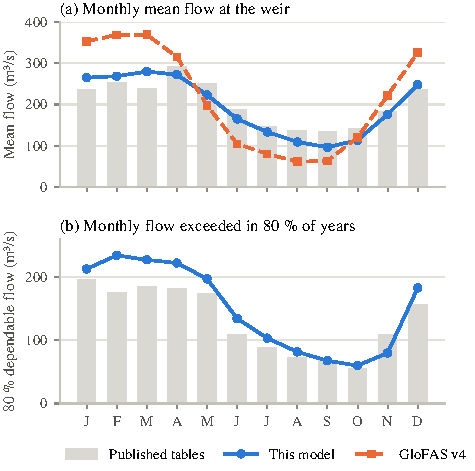
\includegraphics[width=\columnwidth]{figures/fig_rainflow.pdf}
\caption{Modelled flow at the weir against two published tables. (a)~Monthly means: the 1982 study~\citep{jica1982},
our replay of \RepYearFirst--\RepYearLast{} and GloFAS v4. (b)~Monthly flow exceeded in 80~\% of years: the 2022
study~\citep{jica2022} and our replay. The periods of record differ; none of the series is a measurement we hold.}
\label{fig:rainflow}
\end{figure}

\subsection{The weir}

Table~\ref{tab:weir} and Fig.~\ref{fig:weir} show the automatic rule across the flow range. The pond is held at
EL~\PondNormal~m for every inflow up to \PondHeldTo~\cms. Below \EnvFlow~\cms{} the canal gets nothing, because the
river's maintenance flow comes first. Above \PondHeldTo~\cms{} all openings are at the lift where they pass no more
and the pond rises: the design flood of \DesignQ~\cms{} gives EL~\DesignPondAuto~m, \DesignFreeboard~m below design
high water, with a tail level of EL~\DesignTailAuto~m; with every gate fully open and the canal shut the pond is at
EL~\DesignPondOpen~m and the tail at the sourced EL~\DesignTailOpen~m. Design high water is first exceeded at
\PondOverFrom~\cms. The design wave
carries \WaveVolume~\Mm, or \WaveDepth~mm over the catchment. In a sweep from 5 to 3,000~\cms{} in 5~\cms{} steps the
mass balance closes to \BalanceErr{} of the inflow, the pond never jumps by more than \MaxPondJump~m between
neighbouring flows and the tail is never above the pond.

\begin{table}[t]
\caption{The weir under the automatic rule (canal demand \IntakeTarget~\cms). Levels in m EL, lifts in m, flows in
\cms. A range of lifts means the gates are at different openings.}
\label{tab:weir}
\footnotesize\setlength{\tabcolsep}{2.6pt}
\begin{tabularx}{\columnwidth}{@{}rrr>{\raggedright\arraybackslash}Xrrrr@{}}
\toprule
Inflow & Pond & Tail & Stage & Gates & Sluices & Canal & River \\
\midrule
\rows{tab_weir}
\bottomrule
\end{tabularx}
\end{table}

\begin{figure}[t]
\centering
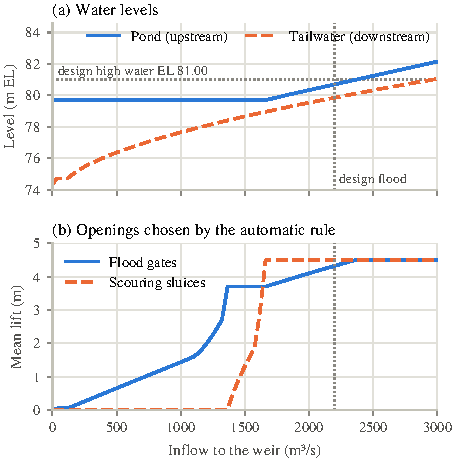
\includegraphics[width=\columnwidth]{figures/fig_weir.pdf}
\caption{Automatic operation against inflow. (a)~Pond and tail levels. (b)~Mean lift of the flood gates and of the
scouring sluices. The plateau of the gates near 1,400--1,650~\cms{} is the lift at which their lips leave the water
and a higher lift passes no more.}
\label{fig:weir}
\end{figure}

\subsection{Flood extent and what it reaches}

The reference level below the weir, EL~\RefTail~m, is the level the tail rating reaches at about \RefFlow~\cms, so
the terrain model saw the river nearly bank-full and smaller floods add no flooded ground. The first cells flood at
\FirstWetQ~\cms{} (Table~\ref{tab:flood}). At the design flood the tail stands \FloodRiseBelowDesign~m and the pond
\FloodRiseAboveDesign~m over their references; \FloodAreaDesign~\kmsq{} of ground is flooded,
\FloodAreaUpDesign~\kmsq{} of it above the weir, with \FloodBldDesign{} buildings in water at least \MinDepth~m deep,
\FloodRoadDesign~km of road and \FloodCropDesign~ha of cropland (Fig.~\ref{fig:flood}). For the 100-year flood the
figures are \FloodAreaQhundred~\kmsq{} and \FloodBldQhundred{} buildings. These counts depend strongly on the one
assumption that cannot be checked from open data, the bank reference: shifting it between $-1.0$ and $+0.5$~m moves
the design-flood area between \SensAreaHi{} and \SensAreaLo~\kmsq{} and the buildings between \SensBldHi{} and
\SensBldLo. The page offers that shift as a slider for this reason.

\begin{table}[t]
\caption{Ground flooded beyond the normal river. Rises in m over the reference below and above the weir; buildings
in water $\geq$\MinDepth~m.}
\label{tab:flood}
\footnotesize\setlength{\tabcolsep}{3pt}
\begin{tabularx}{\columnwidth}{@{}r>{\raggedright\arraybackslash}Xrrrrrr@{}}
\toprule
Flow & Return & \multicolumn{2}{c}{Rise (m)} & Area & Build- & Road & Crop \\
\cms & period & below & above & \kmsq & ings & km & ha \\
\midrule
\rows{tab_flood}
\bottomrule
\end{tabularx}
\end{table}

\begin{figure*}[t]
\centering
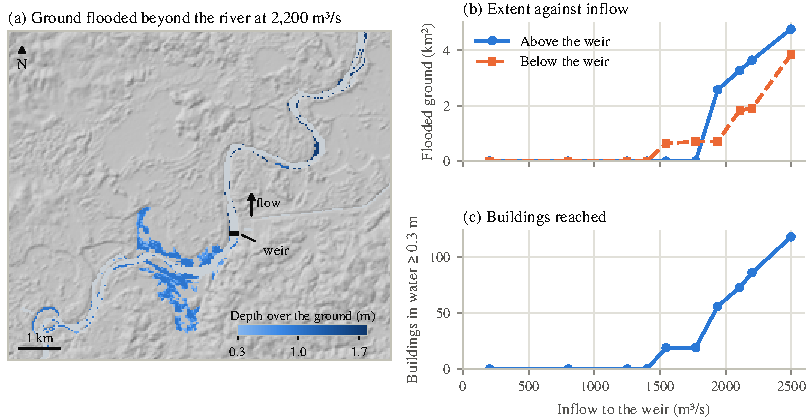
\includegraphics[width=\textwidth]{figures/fig_flood.pdf}
\caption{Flood results. (a)~Depth of water over ground beyond the normal river (grey band) at the design flood,
on the relief of the 30~m surface model; the flooded area above the weir is the pond's rise spreading into a side
valley. (b)~Flooded ground above and below the weir against inflow. (c)~Buildings in water at least \MinDepth~m
deep.}
\label{fig:flood}
\end{figure*}

\subsection{Canal supply}

Demand by half-month peaks at \PeakDR~l/s/ha in \PeakHM, or \PeakDemand~\cms{} on the legal area, against a
published peak of \PeakDRPub~l/s/ha and \PeakDemandPub~\cms{} (Fig.~\ref{fig:ops}a). In the mean year the canal is
never short (\MeanYearShortDays{} days). In the \NDryYears{} driest years of the record it is short on \LeastDryShortDays{} to
\WorstShortDays{} days (Table~\ref{tab:dry}); in \WorstYear, the driest, \WorstShortVol~\Mm{} or \WorstShortPct~\%
of the year's demand of \YearDemandVol~\Mm{} is not delivered, almost all between August and December
(Fig.~\ref{fig:ops}b). In none of these years does the rule let the river below fall under \EnvFlow~\cms{} while
the inflow is above it (\EnvBreachDays{} days).

\begin{table}[t]
\caption{Canal supply by scenario year under the automatic rule. Flows in \cms; shortfall in \Mm.}
\label{tab:dry}
\footnotesize\setlength{\tabcolsep}{3pt}
\begin{tabularx}{\columnwidth}{@{}>{\raggedright\arraybackslash}Xrrrrrr@{}}
\toprule
Year & Rain & Mean & Lowest & Short & Short- & Days \\
 & mm & flow & day & days & fall & met \% \\
\midrule
\rows{tab_dry}
\bottomrule
\end{tabularx}
\end{table}

\subsection{Sediment and the settling basins}

The published rating, used as it stands on the published mean monthly flows, gives \SedUnscaledMt~Mt a year against
a published yield of \SedYieldMt~Mt; the two sourced facts disagree, and we scale the rating's coefficient by
\SedScale{} to match the yield while showing both. With the assumed intake and trap factors, the canal draws
\SedIntakeKt~kt a year (\SedIntakePct~\% of the river's load) at a mean-flow concentration of \SedCmean~mg/l in the
river, and the basins hold back \SedTrapKt~kt (\SedTrapPct~\%). Each basin stores \SedStorage~m$^3$ and is flushed
about every \SedInterval~days, \SedFlushes{} flushes a year in all (Fig.~\ref{fig:ops}c). Every factor in this
paragraph except the rating and the yield is an assumption; the engine shows a mechanism, not a calibrated budget.

\begin{figure*}[t]
\centering
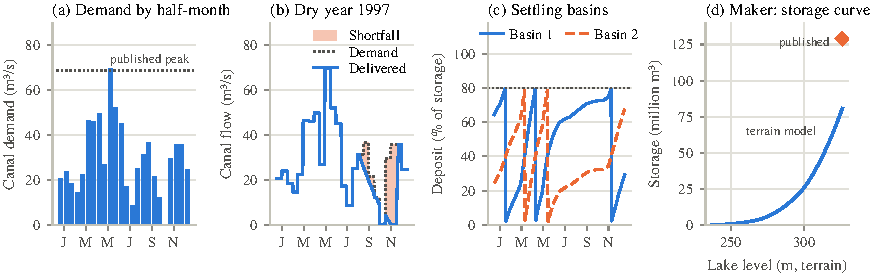
\includegraphics[width=\textwidth]{figures/fig_ops.pdf}
\caption{(a)~Canal demand by half-month on \IrrArea~ha. (b)~Demand and delivery in the driest year of the record.
(c)~Deposits in two of the five settling basins over a mean year; a basin is flushed at \SedFlushAtPct~\%.
(d)~Storage curve of a dam placed at the Tiga Dihaji site, from the terrain model, with the published total
storage.}
\label{fig:ops}
\end{figure*}

\subsection{A dam anywhere}

Two checks show what the terrain grid supports. Catchment tracing is accurate: the weir's catchment comes out at
\CatchGrid~\kmsq{} (\CatchGridErrPct~\% from the published area) and that of the Tiga Dihaji dam site, a dam under
construction upstream, at \TDCatch~\kmsq{} against a published \TDCatchPub~\kmsq~\citep{kurniasari2022}. Volumes are
not: with an assumed full supply level of \TDCrest~m the model lays a dam \TDLen~m long and \TDHeight~m high over the
terrain and finds \TDVol~\Mm{} of storage on \TDArea~\kmsq, only \TDVolPct~\% of the published \TDVolPub~\Mm{}
(height \TDHeightPub~m, crest \TDLenPub~m; Fig.~\ref{fig:ops}d). A surface model measures tree tops, not the valley
floor, the published height is taken from the foundation, and the supply level is our assumption; reservoir volumes
from this tool are therefore a lower bound of unknown tightness. A hypothetical \SelHeight~m dam on the Selabung
(\SelCatch~\kmsq) gives \SelVol~\Mm{} on \SelArea~\kmsq{} and, on the mean year with no release, fills in
\SelFillDays~days.

\section{Verification and limits}

\textbf{Tests.} The repository holds \NTests{} automated tests in \NTestFiles{} files (\NPass{} pass, \NFail{} fail,
\NSkip{} are skipped because they target frequency methods that are not implemented). They include hand-computed
targets for each formula, mass-balance and monotonicity checks, and checks on the real data files: the pond holds
its level across normal flows, the design flood stays under design high water, the mean flow floods nothing.

\textbf{Independent review.} Unit tests did not catch the errors that mattered. A separate review that ran the
whole chain on the real data, after every test had passed, raised sixteen findings, four of them serious: a tail
rating anchored on the wrong level put the design flood 1.7~m above design high water; the automatic rule fed the
canal before the river and left the reach below the weir dry; missing effective rain made irrigation demand 60~\%
too high; and the normal river itself was counted as flood, with more than a hundred buildings ``flooded'' at mean
flow. All four were fixed before release, and each fix is now a test. The review's remaining criticism, the monthly
shape of the flow, stands (Section~5.1). The review is in the repository (\texttt{docs/REVIEW-HYDRAULICS.md}).

\textbf{Limits.} (1)~No gauge record was used. The flow model is fitted to two published tables with different
periods of record, and Lake Ranau's regulated outflow is not modelled separately. (2)~The terrain is a 30~m surface
model with tree tops and roofs in it~\citep{hawker2022}; it cannot see the river bed, dykes or culverts. The flood
map has one rise on each side of the weir, no backwater slope and no timing, and is not a hydraulic flood model.
(3)~The weir's sill, bed and deck levels, the tail section and all sediment factors but two are assumed. (4)~The
pond has no storage: levels answer inflow at once. (5)~Replay years carry seasonal flow, not floods. For these
reasons the page labels every computed value as an indicative model, and nothing here should be used for design,
operation or warning. An information request to the basin authority for the manual, as-built levels and gate logs is
the obvious next step; a bare-earth terrain model~\citep{hawker2022} and a storage term for the pond are the next
changes to the code.

\section{Software and availability}

The page is plain ES modules with no build step: MapLibre~GL~JS~\citep{maplibre} draws the map and hosts a
three.js~\citep{threejs} scene for the structure, the water and the ground. Table~\ref{tab:code} gives the size of
each part. Engines never touch the page; grid work runs in a web worker; modules talk through one store, so each can
be tested alone. On a server core under Node~24 one weir solution takes \SolveMs~ms, a flood extent on the fine grid
\ExtentMs~ms, a catchment trace on the wide grid \CatchMs~ms and a storage curve \CurveMs~ms, which is what makes
dragging a slider feel immediate. The interface is in Indonesian and English.

\begin{table}[t]
\caption{Size of the code and its tests (lines include comments; vendored libraries and language tables are left
out).}
\label{tab:code}
\footnotesize\setlength{\tabcolsep}{4pt}
\begin{tabularx}{\columnwidth}{@{}>{\raggedright\arraybackslash}Xrrr@{}}
\toprule
Part & Files & Lines & Tests \\
\midrule
\rows{tab_code}
\bottomrule
\end{tabularx}
\end{table}

\textbf{Availability.} Code, data files, data-preparation scripts, the build contract the modules were written
against and this paper's source are at \url{\RepoURL} under the MIT licence; third-party data and libraries keep
their own licences (file \texttt{NOTICE.md}). A running copy is at \url{\DemoURL}. \texttt{make} in
\texttt{paper/} reruns the engines and rebuilds every number, table and plot.

\textbf{Use of AI tools.} The simulator's code, its tests, the review pass and the first draft of this text were
produced with AI coding assistants working under the author's direction. The author set the questions, made the
rulings recorded in the build contract, checked the outputs and is responsible for the content.

\section{Conclusion}

A gated weir, its river and its canal can be simulated end to end in a browser from open data alone, at a level
that agrees with published tables to within \QmeanAbsErrPct~\% on annual flow, \RmsMeanPct~\% on monthly flow and
\PeakDRErrPct~\% on peak irrigation demand, and that respects the structure's sourced design levels. The same exercise
shows plainly where open data stop: flood maps and reservoir volumes are bounded by the surface model, and the levels
that matter most inside the structure are not public. Publishing the model with a status letter on every number
makes those boundaries part of the tool.

\bibliographystyle{unsrtnat}
\bibliography{refs}

\appendix
\footnotesize
\section{Calculation details}
\label{app:eq}

\begin{table*}[t]
\caption{Principal parameters. Status: S sourced, C computed, R read from a picture or map, A assumed.}
\label{tab:params}
\scriptsize\setlength{\tabcolsep}{4pt}
\begin{tabularx}{\textwidth}{@{}>{\raggedright\arraybackslash}Xr@{\ \ }c@{\qquad}>{\raggedright\arraybackslash}Xr@{\ \ }c@{}}
\toprule
Parameter & Value & & Parameter & Value & \\
\midrule
\rows{tab_params}
\bottomrule
\end{tabularx}
\end{table*}

Symbols: $P$ rain and $E_0$ reference evapotranspiration (mm/day); $Q$ flow (\cms); $H$, $T$ pond and tail level
(m EL); $g$ gravity. Values and status letters are in Appendix~B; file names refer to \texttt{site/js/engine/}.

\textbf{A.1 Rain to flow} (\texttt{rainflow.js}). Soil store $s$, fast store $f$, slow store $g_s$ (mm), daily step:
\begin{align}
s' &= s+P,\qquad o=\max(0,\,s'-S_{\max}) \label{eq:bucket1}\\
e &= \min\!\Big(s'-o,\;c_eE_0\min\!\big(1,\tfrac{s'-o}{f_cS_{\max}}\big)\Big) \notag\\
f &\leftarrow f+(1-\gamma)\,o,\quad g_s\leftarrow g_s+\gamma\,o,\quad s\leftarrow s'-o-e \notag\\
q &= f\big(1-e^{-1/K_f}\big)+g_s\big(1-e^{-1/K_s}\big)\Big(\frac{g_s}{g_{\mathrm{ref}}}\Big)^{\beta-1} \notag\\
Q &= qA/86.4 \label{eq:bucket3}
\end{align}
with $A$ in \kmsq; each store then loses its outflow. The stores are spun up over three mean years. A design year
adds the wave $w(t)=(Q_p-Q_b)\,(t/t_p)^a\,e^{a(1-t/t_p)}$ to the mean year, with $t_p=\DesignTp$~days,
$a=\DesignShape$ and $Q_p$ read from the published frequency table, interpolated linearly in the Gumbel variate
$-\ln(-\ln(1-1/T))$~\citep{gumbel1958}. Dependable flow uses the Weibull position $m/(n+1)$.

\textbf{A.2 Weir} (\texttt{weir.js}). For a bay of width $b$, sill $z$ and opening $a$, let $h_1=H-z$ and
$h_2=T-z$. Under the leaf
\begin{align}
Q_f &= \mu ab\sqrt{2gh_1},\qquad y_2=\tfrac{y_1}{2}\Big(\sqrt{1+8\mathrm{Fr}_1^2}-1\Big) \label{eq:gate}\\
Q_u &= Q_f\sqrt{\frac{h_1-h_2}{h_1-y_2}}\ \ \text{if } h_2>y_2,\ \text{else } Q_f \notag
\end{align}
where $y_1=\mu a$ is the contracted jet, $\mathrm{Fr}_1$ its Froude number and $y_2$ its conjugate
depth~\citep{henderson1966}. An open bay is a crest:
\begin{align}
Q_c &= C_d\,\tfrac23\sqrt{\tfrac23g}\;B_e\,h_1^{3/2}\Big(1-\big(h_2/h_1\big)^{3/2}\Big)^{0.385} \label{eq:crest}\\
B_e &= b-2\,(nK_p+K_a)\,h_1 \notag
\end{align}
and the bay passes $\min\!\big(Q_u,\;Q_c\,(a/h_1)^{1/2}\big)$, a continuous hand-over that is our own numerical
choice. Water over the top of a leaf is a crest with head $H-(z+a+h_{\mathrm{leaf}})$. The intake passes
$Q_i=\mu_ib_ia_i\sqrt{2g(H-H_c)}$, capped by demand and capacity. Below the weir~\citep{chow1959}
\begin{align}
Q &= \frac1n\,A_x^{5/3}P_x^{-2/3}S^{1/2},\qquad T=z_t+y \label{eq:manning}\\
A_x &= (b_t+m y)\,y,\qquad P_x=b_t+2y\sqrt{1+m^2} \notag
\end{align}
The pond level solves $Q_{in}-Q_i(H)-\sum_k Q_k(H,T)=0$ by bisection, with $T$ such that Eq.~\ref{eq:manning}
carries $\sum_kQ_k$. In automatic mode $Q_i=\min(D,\,Q_{cap},\,\max(0,Q_{in}-Q_{env}))$ and the openings are found
by bisection along the operating sequence so that the structure passes $Q_{in}-Q_i$ at the normal pond $H_n$; past
the last stage they rise to full lift in proportion to $(H-H_n)/(H_d-H_n)$, $H_d$ being design high water.

\textbf{A.3 Flood and impact} (\texttt{flood.js}, \texttt{impact.js}). Let $M$ be the main river: the D8 path below
the weir and the drainage cells above it with at least 1,000~\kmsq{} upstream. Let $r(c)$ be the first cell of $M$
on the D8 path of cell $c$ and $h_M(c)=z_c-z_{r(c)}$. With the rise $s=\max(0,T-T_{\mathrm{ref}})$ for cells that
drain to the river below the weir and $s=\max(0,H-H_n)$ for cells that drain through it, a cell is wet when
\begin{equation}
h_M(c)\le s-d_{\min}\quad\text{and it joins } M \text{ through wet cells;}\qquad d_c=s-h_M(c) \label{eq:flood}
\end{equation}
(eight neighbours), followed by one $3\times3$ majority pass. Cells of permanent water or inside the river outline
carry the connection but are never returned. Areas are sums of the ellipsoidal area of each cell. Buildings are
indexed by map tile; a building counts when its point lies in a wet cell at least $d_{\min}$ deep. Road and rail
lengths are clipped to wet cells, bridges left out.

\textbf{A.4 Irrigation} (\texttt{irrigation.js}). Per half-month, with percolation $P_c$, water-layer replacement
$W$ and effective rain $R_e=0.7R_{80}/15$:
\begin{align}
\mathit{NFR}_{\mathrm{lp}} &= \frac{M e^{k}}{e^{k}-1}-R_e,\quad M=1.1E_0+P_c,\quad k=\frac{MT}{S} \label{eq:nfr}\\
\mathit{NFR} &= K_cE_0+P_c+W-R_e,\qquad \mathit{DR}=\frac{\mathit{NFR}}{8.64\,e} \label{eq:dr}
\end{align}
for land preparation and growth, in mm/day and l/s/ha, averaged over the groups; the dry-season crop has
$\mathit{NFR}=K_cE_0-R_e$. The intake demand is $\mathit{DR}$ times the area.

\textbf{A.5 Sediment} (\texttt{sediment.js}). $Q_s=aQ^b$ (t/day), with $a$ scaled so that the mean monthly flows
carry the yield $Y$; concentration $C=10^6aQ^{b-1}/86400$~mg/l. Each of the $n$ basins not being flushed receives
$q=Q_i/n$ at concentration $\kappa C$ and gains deposit volume at the rate
\begin{align}
\frac{dV}{dt} &= \frac{\eta\,q\,\kappa C}{\rho_d} \label{eq:sed}\\
\eta &= \big[\sigma\eta_s+(1-\sigma)\eta_f\big]\,\min\!\big(1,\tfrac{q_d}{q}\big)\,\phi(F) \notag
\end{align}
with $F$ the fill and $\phi$ falling linearly from 1 at $F=0.8$ to 0 at $F=1$; the $q_d/q$ term follows Hazen's
surface-loading argument~\citep{hazen1904}. A flush empties a basin as $V\leftarrow Ve^{-\lambda t}$ to 2~\% in
\SedFlushHours~hours, slowed when the river has no water to spare. Steps are cut to 15~minutes at most.

\textbf{A.6 Terrain and reservoir} (\texttt{grid.js}, \texttt{reservoir.js}). A catchment is the set of cells whose
D8 path passes the outlet, found by a breadth-first search upstream. The dam line is marched from the snapped cell
in half-cell steps, both ways, until the ground reaches the crest. The pond is a priority flood from a seed just
upstream of the dam line, four-connected, that stops at the crest or at the first cell from which water would
escape (round the dam or off the grid). Over the pond's cells, sorted by ground level,
\begin{align}
V(h) &= \sum_{z_c<h}A_c\,(h-z_c),\qquad A(h)=\sum_{z_c<h}A_c \label{eq:curve}\\
V_2 &= V_1+\Delta t\Big[\tfrac{I_1+I_2}{2}-\tfrac{O(V_1)+O(V_2)}{2}\Big] \label{eq:puls}\\
O &= Q_r+C_sB_s\,(h-h_c)^{3/2}+E\,A(h) \notag
\end{align}
the second being level-pool (modified Puls) routing, solved for $V_2$ by bisection.

\section{Parameters}
\label{app:params}

Table~\ref{tab:params} lists \NParamsShown{} of the \NParams{} engine parameters with the status of each, read from
\texttt{site/data/params.json} when the paper is built.


\section{Software and data preparation}
\label{app:soft}

\textbf{C.1 Structure.} \texttt{site/} is the whole application: plain ES modules loaded in a fixed order, with no
bundler and no network request to any other host. Every module exports one \texttt{init(ctx)}. Modules never import
each other across the user-interface, map and simulation groups; they talk through one store with dotted keys
(\texttt{flow.q\_in}, \texttt{weir.pond\_el}, \texttt{flood.area\_km2}, \dots) and through named fields for large
arrays such as the flood mask. The engines (Table~\ref{tab:code}) have no access to the page. Light ones are called
directly by the simulation runner; those that need a terrain grid run in a web worker, called as
\texttt{engine.call('flood.extent', args)}, with typed arrays transferred rather than copied. Each step of the
runner reads the scenario's flow for the date, asks the irrigation engine for the canal demand, solves the weir,
updates the irrigation balance and the settling basins, and, when a rise has moved by 0.1~m, recomputes the flood
extent and the impact count.

\textbf{C.2 Drawing.} A MapLibre custom layer shares its WebGL context with one three.js scene in metres at true
scale. The weir, its gates, the intake, the settling basins and maker-mode dams are built from the geometry file by
factory functions that never touch the map. The water in each bay is a surface shaped from that bay's computed
flow, opening and levels (the jet under the leaf, the hydraulic jump, the pool behind the end sill); river sheets
follow a flow field traced along the channel. This layer draws what the engines computed and returns no number to
them. The in-page recorder steps the simulation by exactly 1/30~s per frame and encodes H.264 with WebCodecs, so a
film is the same on any machine.

\textbf{C.3 Data files.} A terrain grid is a JSON header and raw little-endian arrays, row-major from the
north-west corner: elevation (Int16, decimetres), D8 direction (Uint8), upstream area (Float32, \kmsq), height
above drainage (Int16, decimetres) and land cover (Uint8). Buildings are Float32 triplets (longitude, latitude,
footprint area) sorted by a zoom-12 tile key with an index. Terrain tiles are Terrarium-coded PNGs. Facts and
parameters are JSON leaves of the form \{value, unit, status, sources\}, assembled from fragments by
\texttt{tools/data/build.mjs} and checked by \texttt{tools/data/check.mjs}.

\textbf{C.4 Preparation} (\texttt{tools/dataprep/}; band 2 of Fig.~\ref{fig:pipeline}). Six GLO-30 tiles were mosaicked; pits and depressions were
filled and flats resolved; mapped rivers were burned in by 20~m where the surface lies under 120~m, and Lake Ranau
was set flat. The wide grid averages $3\times3$ cells; the fine grid keeps the 1-arc-second cells and takes its
inflow from the wide grid. Height above drainage uses channels of at least 200~\kmsq{} (wide) and 50~\kmsq{}
(fine); the flood engine recomputes it against the main river only. At the weir the terrain tiles were carved to the
assumed bed so that a true-scale structure can stand in the river. The river outline is a water-index threshold on
a Sentinel-2 scene of 26 April 2026. Land cover is the majority class per cell. Basin rain is the equal-weight mean
of the ERA5 cells returned for a $4\times3$ grid of points.

\textbf{C.5 Reproducing the paper.} Node 22 or later, Python 3 with numpy and matplotlib, and \LaTeX.
{\scriptsize
\begin{verbatim}
node tools/serve.mjs --port 8791  # the simulator
npm test                          # the tests
cd paper && make                  # numbers, plots, PDF
\end{verbatim}
}

\end{document}
